\documentclass[12pt,a4paper]{report}
\usepackage[margin=1in]{geometry}
\usepackage[T1]{fontenc}
\usepackage[utf8]{inputenc}
\usepackage{setspace}
\usepackage{amsmath}
\usepackage{amssymb}
\usepackage{graphicx}
\usepackage{booktabs}
\usepackage{longtable}
\usepackage{xcolor}
\usepackage{hyperref}
\usepackage{listings}
\usepackage{fancyhdr}

\onehalfspacing
\graphicspath{{../figures/}}
\pagestyle{fancy}
\fancyhf{}
\lhead{Streaming WFC Final Report}
\rhead{\thepage}

\lstset{
  basicstyle=\ttfamily\small,
  frame=single,
  breaklines=true,
  columns=fullflexible
}

\title{\textbf{Streaming Procedural Terrain Generation with Wave Function Collapse}\\
\large Final Project Report for Algorithms Design and Analysis}
\author{Saugat Shakya\\
M.Sc. Data Science and Artificial Intelligence\\
Asian Institute of Technology}
\date{April 9, 2026}

\begin{document}
\maketitle
\tableofcontents
\clearpage

\begin{abstract}
This report presents the final version of a streaming terrain generator built around Wave Function Collapse (WFC) and implemented as a local browser demo plus a headless experiment pipeline. The project goal was to turn an initially proposal-level idea into a coherent masters-level algorithms project with a truthful implementation story, a presentable live demonstration, and a reproducible experiment package. The final system uses an XML-driven Summer tileset, propagator-based boundary restriction, halo-conditioned chunk solving, persistence through storage-backed chunk reloads, and a pure backtracking streaming path. A separate controlled experiment harness retains restart-mode WFC only for comparison purposes.

The final measurements show that the system is fully functional as a streaming generator. In the controlled comparison, backtracking outperformed restart on mean solve time at every tested size: $3.84$ ms versus $8.53$ ms at $10 \times 10$, $32.28$ ms versus $114.29$ ms at $20 \times 20$, and $318.72$ ms versus $867.14$ ms at $30 \times 30$. Backtracking solved all $10 \times 10$ and $20 \times 20$ instances within the 5 s experimental cap and solved $97\%$ of $30 \times 30$ instances, with the remaining $3\%$ recorded as timeouts. In streaming scenarios, the final demo path achieved zero seam violations, zero internal violations, and perfect revisit consistency across all tested chunk sizes. The measured mean per-generated-chunk times were $8.29$ ms at $10 \times 10$, $52.01$ ms at $20 \times 20$, and $205.95$ ms at $30 \times 30$.

The project therefore succeeds as a working streaming WFC system and as an algorithms analysis project. The most important final conclusion is not simply that the code runs, but that the full package now aligns the demo, experiments, report, and presentation around one consistent and reproducible implementation.
\end{abstract}

\chapter{Introduction}
The original proposal aimed to build an ``infinite'' terrain generator using Wave Function Collapse. During implementation, the project evolved from a general architectural idea into a concrete systems-and-algorithms artifact with three final deliverables:

\begin{enumerate}
\item a stable local-browser demo for streaming terrain generation,
\item a reproducible headless experiment package for algorithm comparison and system validation,
\item a final report and presentation package that accurately describe the implemented system.
\end{enumerate}

The key challenge is that vanilla WFC is naturally formulated for a bounded offline grid, while the target application here is an online system that must extend a partially committed world. Once a player has observed terrain, those assignments cannot be discarded. This project therefore reformulates streaming terrain generation as an \textbf{incremental constraint satisfaction problem}: each new chunk must be generated as a consistent extension of already committed neighboring chunks, while preserving revisit identity and staying fast enough for an interactive demo.

\section*{Final Claim}
The final claim of the project is narrower and stronger than the original proposal: \textbf{a pure-backtracking streaming WFC system can deliver a reliable interactive demo with correct seams and deterministic revisit behavior, and it compares favorably against restart-mode WFC on controlled isolated benchmarks.}

\chapter{Problem Definition}
\section{World Model}
The world is partitioned into square chunks of size $G \times G$. Each cell stores one tile from a finite tile alphabet derived from the Summer XML tileset. The active viewport only shows a small window into the world, so chunks are generated on demand and evicted from memory when no longer needed.

\section{Correctness Requirements}
The project is evaluated against three explicit requirements.

\begin{enumerate}
\item \textbf{Seam correctness:} tiles on chunk borders must remain compatible with tiles in adjacent chunks.
\item \textbf{Internal correctness:} all tile adjacencies inside each chunk must satisfy the same constraints.
\item \textbf{Temporal consistency:} revisiting a location after eviction and reload must recover exactly the same tile assignment.
\end{enumerate}

\section{Why Standard WFC Is Insufficient}
Standard WFC solves a single bounded region and typically handles contradictions by restarting from scratch. That policy is incompatible with a streaming world because:

\begin{enumerate}
\item already committed neighboring chunks cannot be discarded,
\item runtime variance from repeated restart attempts creates unstable latency,
\item boundary cells must be solved under fixed external constraints rather than from an unconstrained empty grid.
\end{enumerate}

\chapter{Design Evolution}
\section{Initial Proposal vs Final Implementation}
Several parts of the proposal changed during implementation:

\begin{enumerate}
\item The final project uses the Summer XML ruleset directly rather than performing image-based rule extraction.
\item The live streaming path uses \textbf{pure backtracking only}. Restart mode is retained only inside the headless comparison harness.
\item The solver implementation was rewritten from clone-based search to explicit \textbf{change-record undo backtracking}, which now matches the algorithmic explanation in this report.
\item The final experiment package is driven by the canonical JSON bundle in [\texttt{experiments/streaming\_wfc\_experiment\_bundle.json}].
\end{enumerate}

\section{Boundary-Seeding Failure}
The first concrete implementation problem appeared at chunk boundaries. A naive direct-copy strategy attempted to force border cells in the new chunk to match already committed neighbor values exactly. This fails at corner cases because a single cell can be constrained by two different neighbors simultaneously.

The final experiment bundle records a deterministic reproduction:

\begin{itemize}
\item left committed tile id = 0,
\item top committed tile id = 1,
\item direct hard assignment would require the same target cell to hold both values,
\item propagator-based restriction yields a non-empty allowed set \{9\}.
\end{itemize}

The important lesson is that boundary integration must remain a domain-restriction process, not a direct overwrite of cell values.

\section{Final Boundary Strategy}
The final seeding strategy uses the propagator directly. For a cell $x$ adjacent to a committed neighbor tile $t$ in direction $d$, the domain is restricted to:
\[
D(x) \leftarrow D(x) \cap \{u \mid u \text{ is compatible with } t \text{ in direction } d\}.
\]

This preserves all legal assignments instead of forcing a potentially inconsistent single value.

\section{Halo Conditioning}
The final runtime still uses halo-based region solving: the solver works on a slightly expanded region and commits only the central chunk core. In implementation terms, this reduces pressure at artificial chunk borders by giving propagation a small buffer. The final empirical ablation, however, is mixed rather than uniformly positive. On the specific capped benchmark used in this report, the halo increased time and did not improve success rate. This result is reported honestly in Chapter 7 and treated as a design finding rather than hidden.

\chapter{Final System}
\section{Runtime Architecture}
The cleaned final project keeps the live runtime files in the repository root:

\begin{itemize}
\item \texttt{index.html}
\item \texttt{app.js}
\item \texttt{world.js}
\item \texttt{solver.js}
\item \texttt{rules.js}
\item \texttt{renderer.js}
\item \texttt{validators.js}
\item \texttt{stats.js}
\item \texttt{rng.js}
\item \texttt{tiles/}
\end{itemize}

Supporting artifacts are organized into \texttt{report/}, \texttt{experiments/}, \texttt{figures/}, and \texttt{archive/}.

\section{Demo Preset}
The final browser demo is locked to a stable presentation preset:

\begin{itemize}
\item world seed: \texttt{20260330}
\item chunk size: \texttt{10}
\item viewport: \texttt{8 x 8}
\item storage enabled
\item validation counters visible in the live stats panel
\end{itemize}

\begin{figure}[h]
\centering
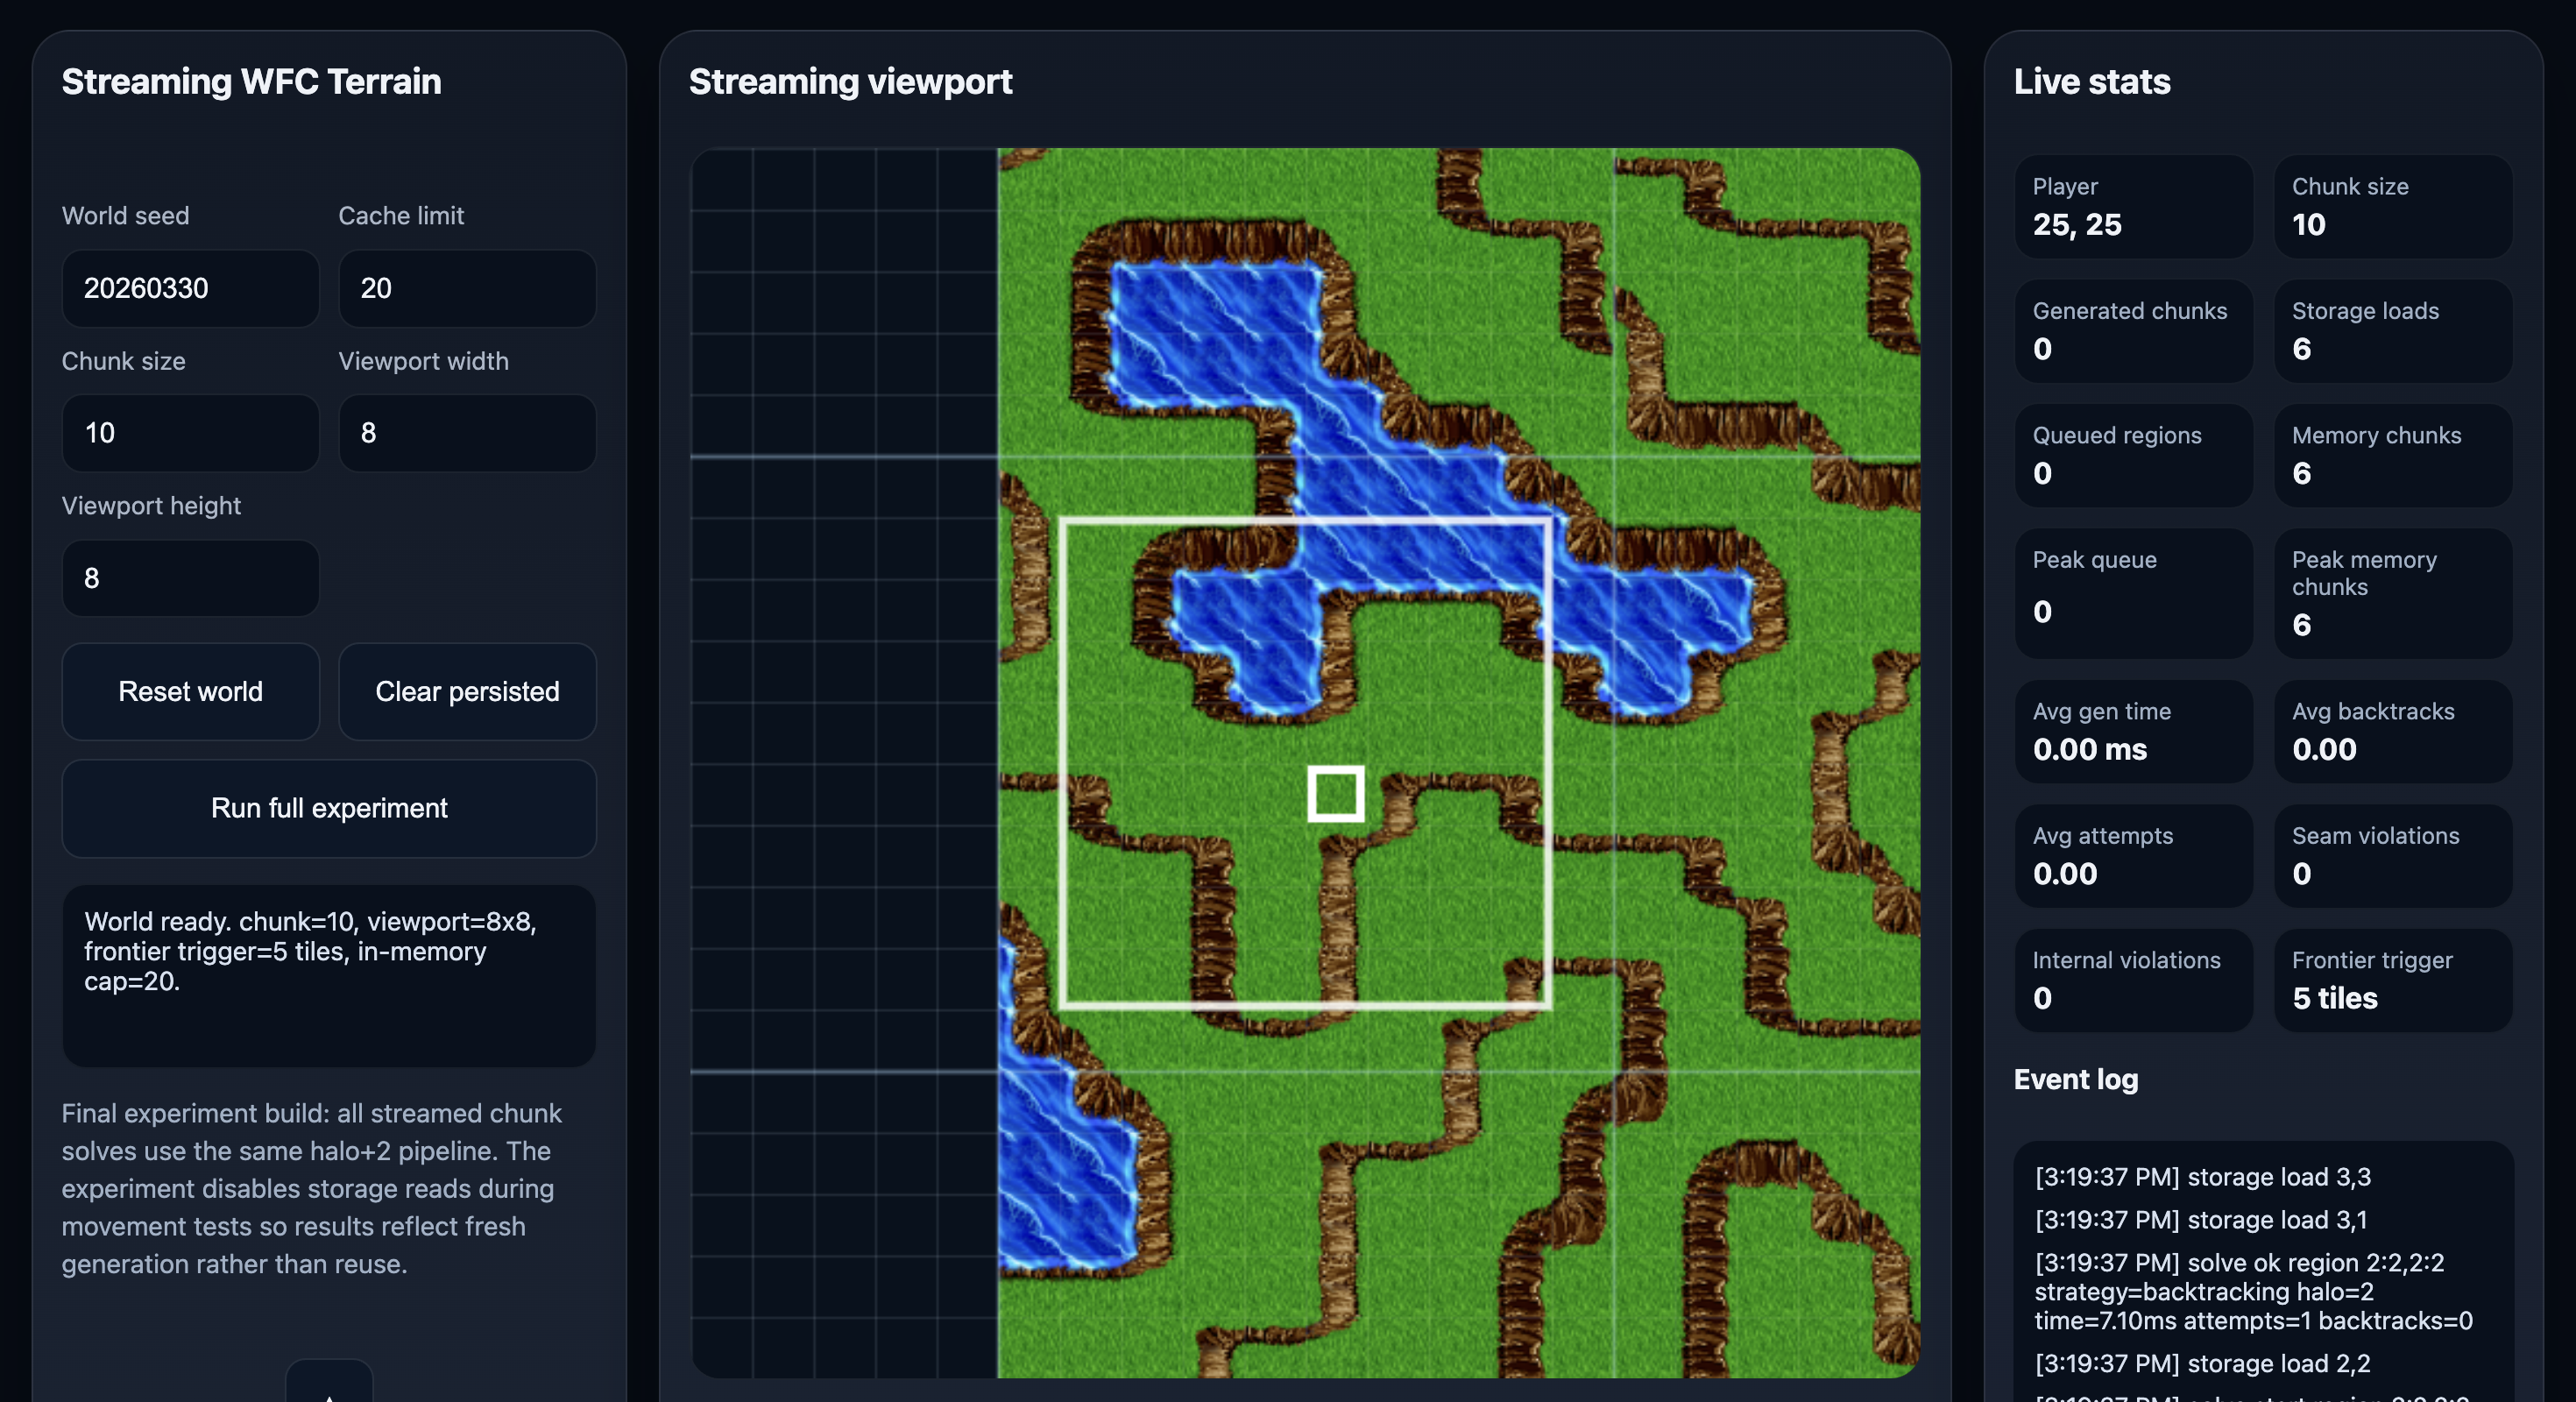
\includegraphics[width=\textwidth]{screenshot.png}
\caption{Final browser demo layout with controls, streaming viewport, validation metrics, and event log.}
\end{figure}

\section{Pipeline}
\begin{figure}[h]
\centering
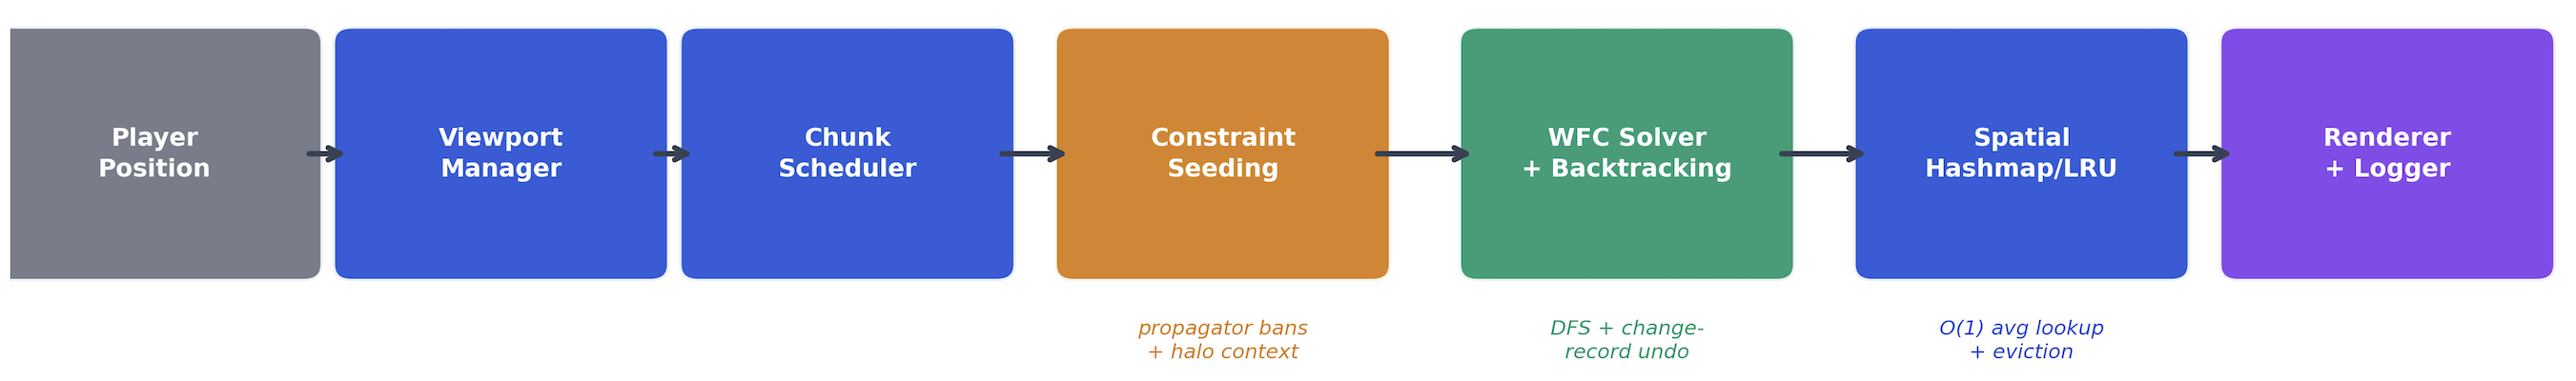
\includegraphics[width=0.8\textwidth]{fig04_pipeline.png}
\caption{Final pipeline: player motion updates viewport demand, missing regions are seeded from committed neighbors, solved, validated, persisted, and rendered.}
\end{figure}

At a high level, the runtime loop is:

\begin{enumerate}
\item detect newly visible or frontier chunks,
\item build boundary restrictions from committed neighbors,
\item solve the requested region with backtracking,
\item validate seams and internal adjacencies,
\item persist the chunk and update cache state,
\item reload evicted chunks from storage on revisit.
\end{enumerate}

\chapter{Algorithms and Data Structures}
\section{Pure Backtracking Solver}
The final solver chooses the unresolved cell with minimum entropy, branches over its currently legal tiles, applies propagation, and undoes changes in reverse order on failure. The solver records changes rather than cloning the entire state for each recursive branch.

\begin{lstlisting}
solve(state):
  apply seeded domain restrictions
  return dfs(state)

dfs(state):
  if every cell is resolved:
    return success

  cell <- minimum entropy unresolved cell
  for tile in ordered legal tiles(cell):
    changes <- collapse cell to tile and propagate
    if propagation succeeds:
      if dfs(state) succeeds:
        return success
    undo(changes)

  return failure
\end{lstlisting}

\section{Streaming Generation Procedure}
\begin{lstlisting}
stream_step(player_move):
  update player position and movement direction
  queue newly visible chunks immediately
  queue frontier chunks when boundary distance is small
  for each queued region:
    build seeded halo region from committed neighbors
    solve region with backtracking
    validate chunk core
    save solved chunk to memory and storage
  evict non-essential chunks from memory
\end{lstlisting}

\section{Primary Data Structures}
\begin{center}
\begin{tabular}{llll}
\toprule
Structure & Purpose & Key Operation & Cost \\
\midrule
\texttt{Map<cx,cy,chunk>} & chunk cache & lookup / insert & $O(1)$ avg \\
\texttt{wave[cell][tile]} & domain state & ban / restore & $O(1)$ \\
\texttt{compatible[cell][tile][dir]} & support counts & decrement / restore & $O(1)$ \\
\texttt{counts[cell]} & domain cardinality & entropy filtering & $O(1)$ \\
change record list & undo log & reverse replay & $O(|\Delta|)$ \\
\texttt{localStorage} backing & persistence & save / reload & $O(G^2)$ per chunk \\
\bottomrule
\end{tabular}
\end{center}

\section{Complexity}
Let $n=(G+2h)^2$ be the halo-expanded local region size and let $|D|=40$ be the tile alphabet size.

\begin{itemize}
\item Cell selection is a linear scan over unresolved cells: $O(n)$.
\item A single propagation step costs $O(|\Delta_k|)$ where $|\Delta_k|$ is the number of actual bans and support-count updates triggered by the current collapse.
\item Undo cost is also $O(|\Delta_k|)$ because only touched entries are restored.
\item Worst-case search time remains exponential, $O(|D|^n)$, because the solver is complete.
\item Active world memory is $O(C \cdot G^2)$ where $C$ is the chunk cache limit.
\end{itemize}

The important design point is that practical performance depends on how fast propagation collapses the domain space, not on the pessimistic worst-case bound alone.

\chapter{Experimental Methodology}
\section{Canonical Bundle}
All reported numbers come from:
\[
\texttt{experiments/streaming\_wfc\_experiment\_bundle.json}
\]
generated on April 9, 2026.

\section{Environment}
\begin{itemize}
\item world seed: \texttt{20260330}
\item tileset: Summer XML
\item controlled comparison sizes: $10 \times 10$, $20 \times 20$, $30 \times 30$
\item controlled runs per condition: 100
\item restart cap: 160 attempts
\item isolated-solve time cap: 5 s per solve
\item streaming viewport: $8 \times 8$
\item streaming paths: 240, 180, and 72 moves for $10$, $20$, and $30$
\item halo ablation runs: 50 per size per halo setting
\end{itemize}

\section{Metric Definitions}
\begin{itemize}
\item \textbf{success rate}: fraction of runs that produced a valid solved grid within the configured cap,
\item \textbf{timeout rate}: fraction of runs that hit the 5 s controlled-solve cap,
\item \textbf{avg generation time}: mean measured solve time recorded by the solver metrics,
\item \textbf{seam/internal violations}: validator failures after chunk generation,
\item \textbf{revisit consistency}: equality of sampled tile values before and after forced eviction and reload.
\end{itemize}

\chapter{Results}
\section{Controlled Backtracking vs Restart}
Table~\ref{tab:comparison} summarizes the isolated solver comparison. The headline result is straightforward: backtracking was faster than restart at all sizes, and restart required more attempts as size increased.

\begin{table}[h]
\centering
\small
\begin{tabular}{rrrrrrrr}
\toprule
Size & BT success & BT timeout & BT mean ms & BT p95 ms & RS success & RS mean ms & RS mean attempts \\
\midrule
$10 \times 10$ & 100\% & 0\% & 3.84 & 5.55 & 100\% & 8.53 & 1.14 \\
$20 \times 20$ & 100\% & 0\% & 32.28 & 38.52 & 100\% & 114.29 & 1.59 \\
$30 \times 30$ & 97\% & 3\% & 318.72 & 157.93 & 100\% & 867.14 & 3.02 \\
\bottomrule
\end{tabular}
\caption{Controlled comparison with 100 runs per size and a 5 s cap per isolated solve.}
\label{tab:comparison}
\end{table}

Additional interpretation:

\begin{itemize}
\item At $10 \times 10$, backtracking is more than twice as fast as restart and keeps attempts fixed at 1.0.
\item At $20 \times 20$, restart remains correct but becomes substantially slower and more variable.
\item At $30 \times 30$, backtracking remains faster on average but develops a long tail; 3 runs hit the 5 s cap, while restart solved all runs with a higher mean time and mean attempts above 3.
\end{itemize}

\begin{figure}[h]
\centering
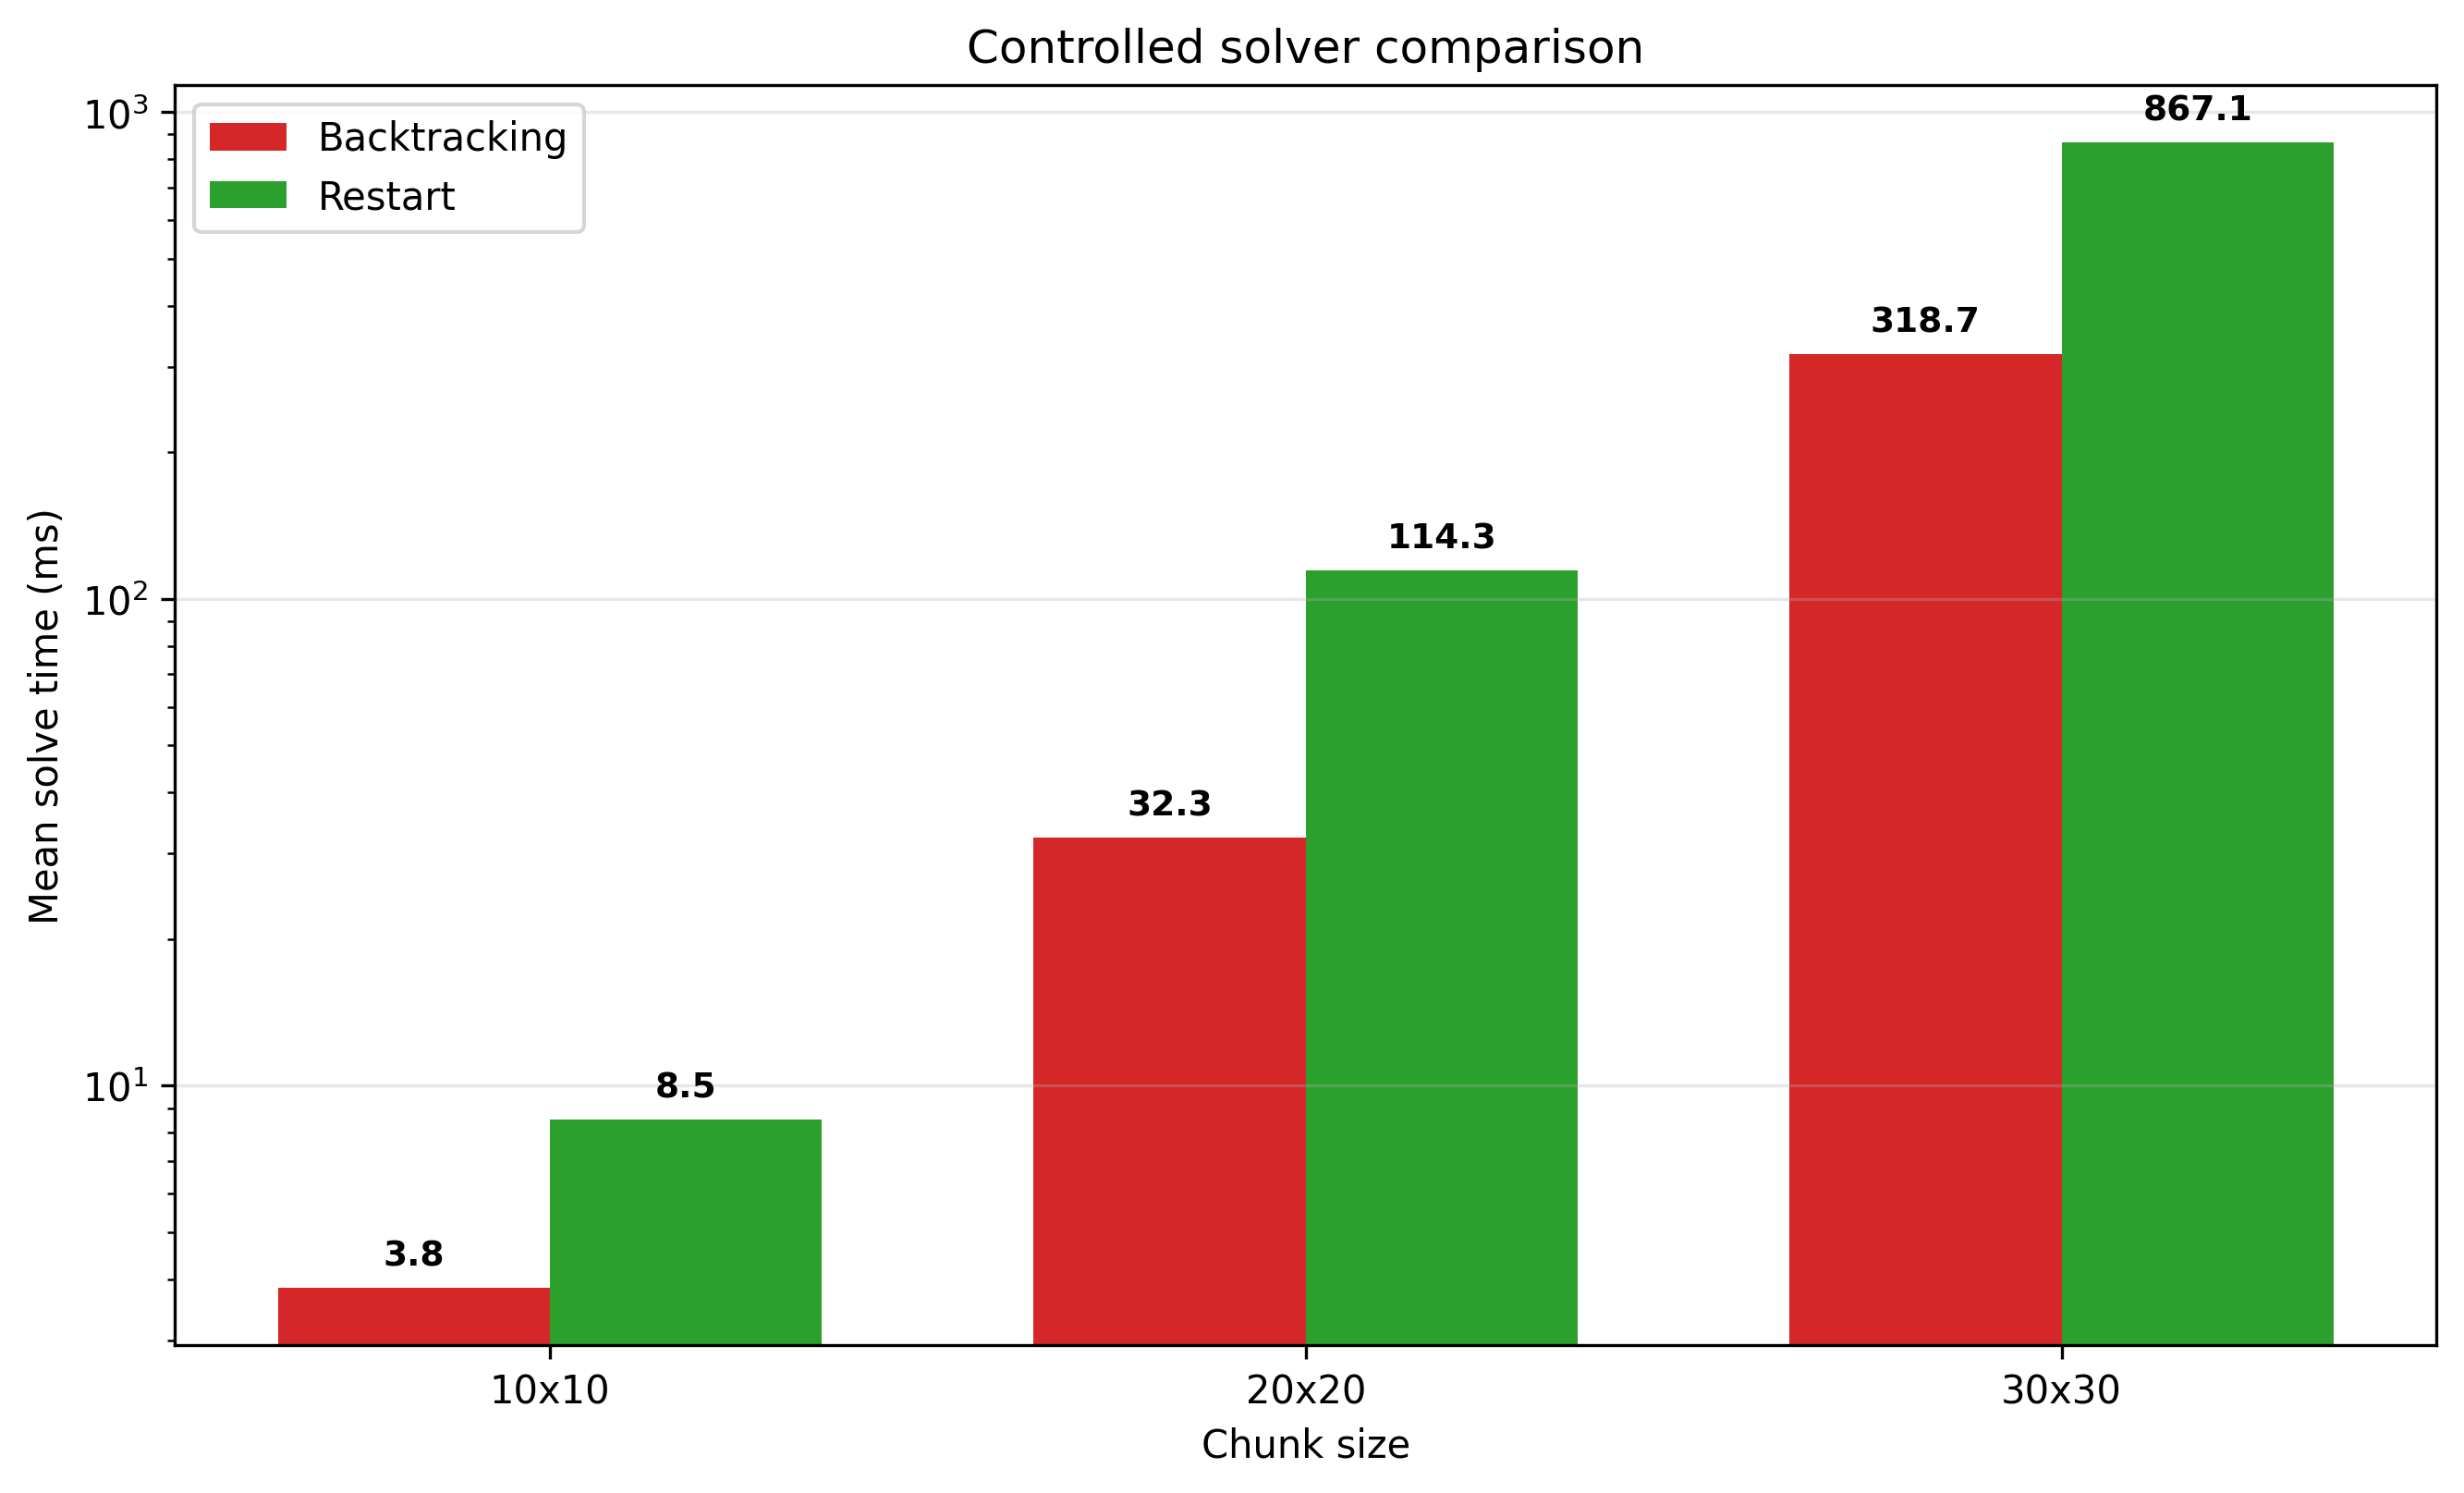
\includegraphics[width=0.85\textwidth]{fig_bt_vs_restart_timing.png}
\caption{Mean time comparison for backtracking and restart in the controlled benchmark.}
\end{figure}

\begin{figure}[h]
\centering
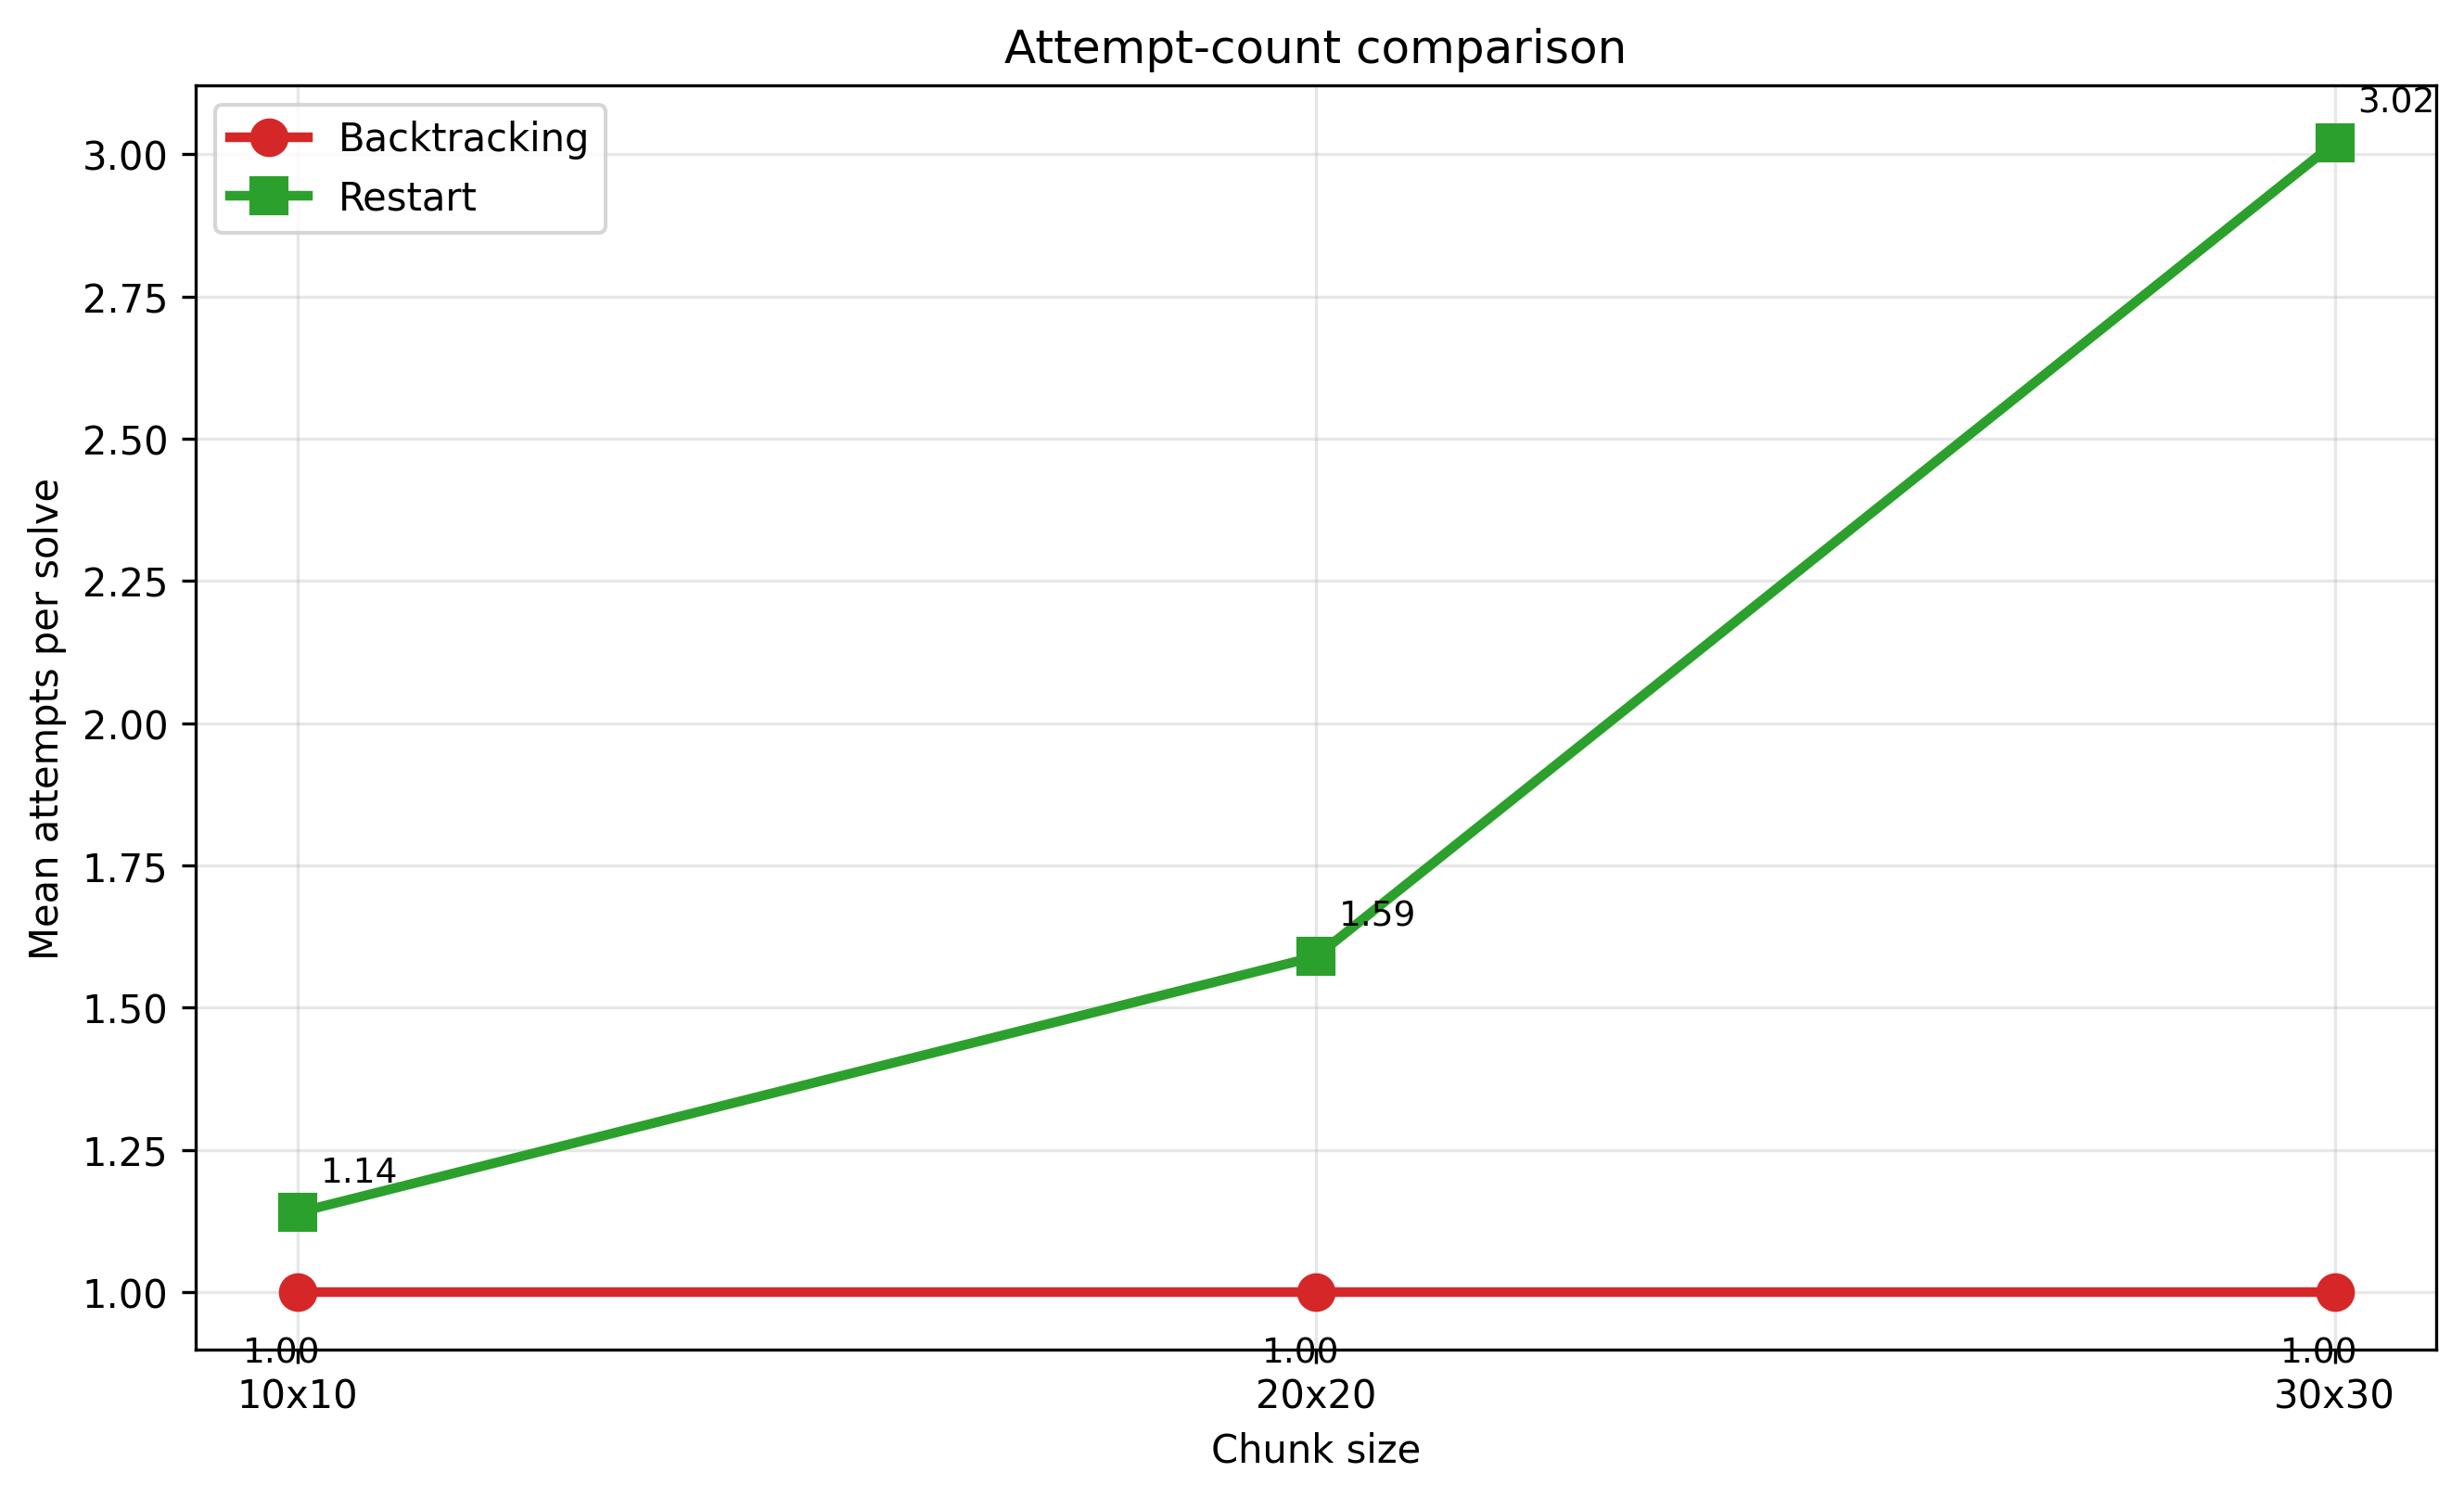
\includegraphics[width=0.85\textwidth]{fig_attempt_count_comparison.png}
\caption{Mean attempt counts. Backtracking stays at 1.0 by construction; restart effort increases with problem size.}
\end{figure}

\begin{figure}[h]
\centering
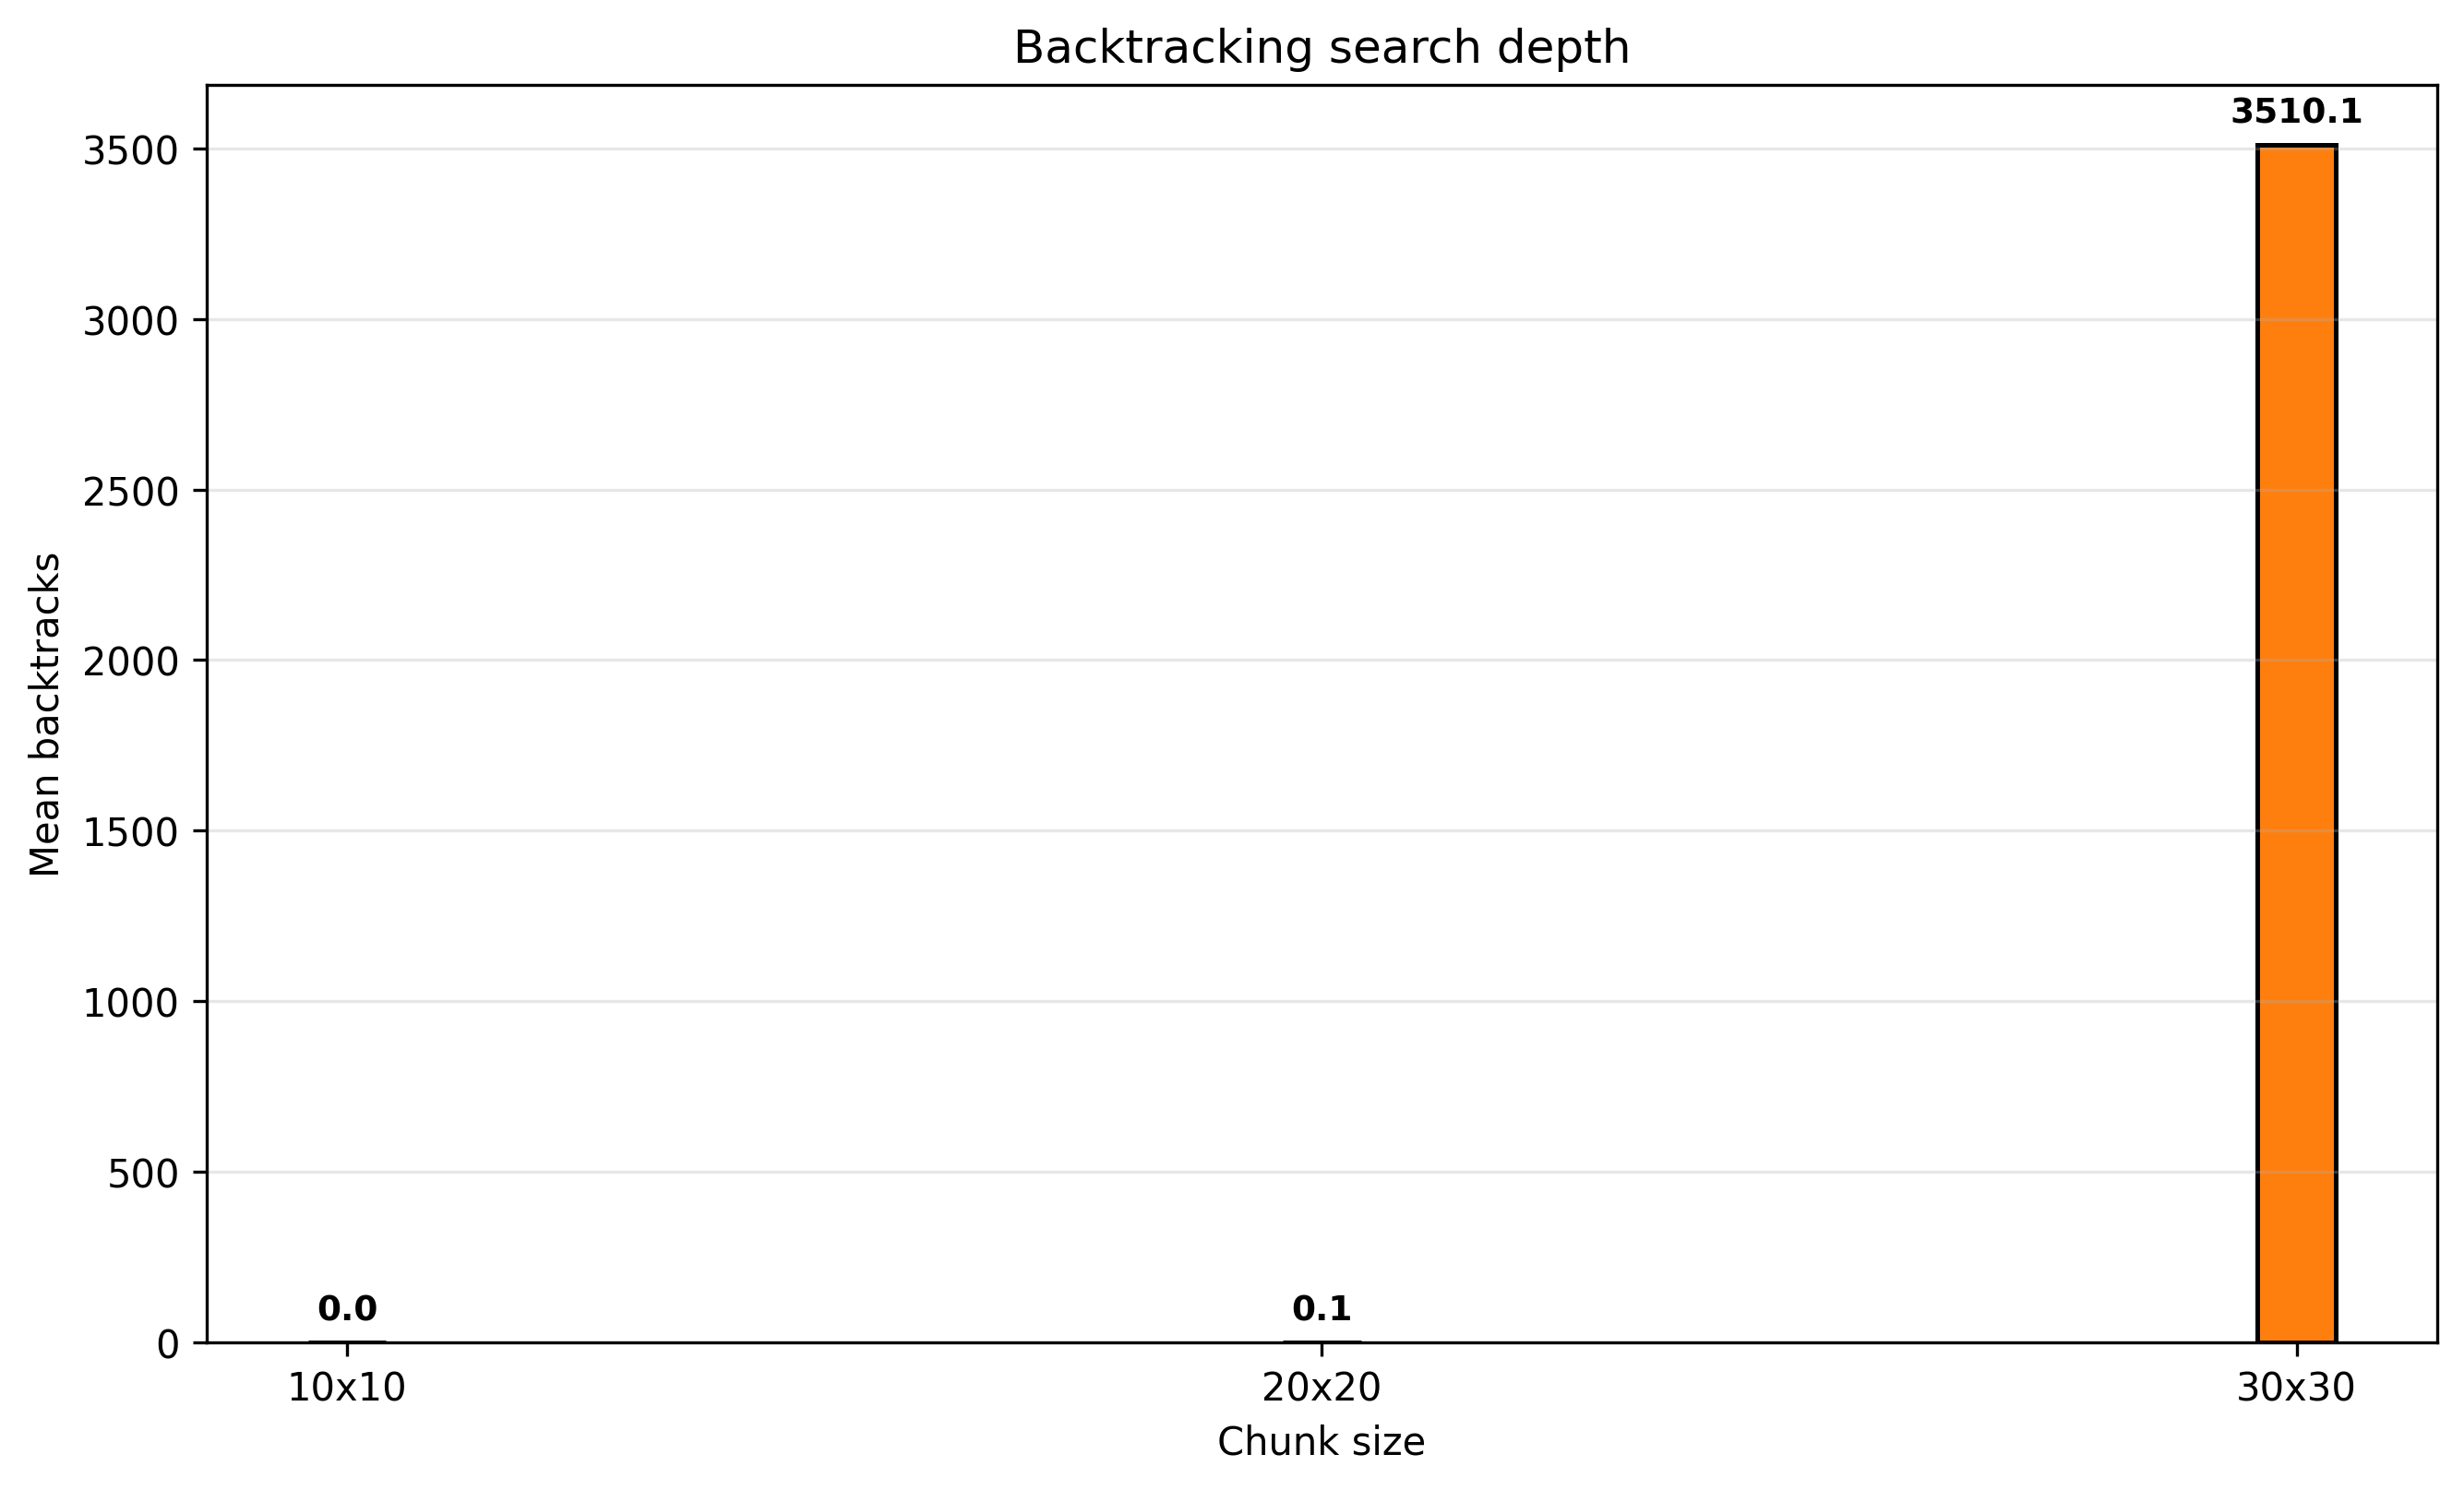
\includegraphics[width=0.85\textwidth]{fig_backtrack_depth.png}
\caption{Mean backtrack counts for the controlled backtracking solver. The heavy tail at $30 \times 30$ explains the wide timing variance.}
\end{figure}

\section{Streaming Scenarios}
The streaming scenarios are the most important system-level result because they use the actual world manager, persistence path, and validators.

\begin{table}[h]
\centering
\small
\begin{tabular}{rrrrrrrr}
\toprule
Size & Moves & Chunks & Mean ms & Attempts & Mean BT & Seam V. & Revisit \\
\midrule
$10 \times 10$ & 240 & 33 & 8.29 & 1.0 & 55.33 & 0 & pass \\
$20 \times 20$ & 180 & 23 & 52.01 & 1.0 & 1.00 & 0 & pass \\
$30 \times 30$ & 72 & 7 & 205.95 & 1.0 & 0.00 & 0 & pass \\
\bottomrule
\end{tabular}
\caption{Streaming scenario results. Internal violations were also zero in every scenario.}
\end{table}

Important observations:

\begin{itemize}
\item The demo target configuration, $10 \times 10$, remains comfortably interactive at 8.29 ms mean solve time.
\item All three scenarios produced zero seam violations and zero internal violations.
\item All three revisit tests passed after forced eviction; the total number of storage reloads added by the revisit checks was 68.
\item The system therefore meets the strongest software claim of the project: it behaves correctly as a streaming world, not just as an isolated solver.
\end{itemize}

\begin{figure}[h]
\centering
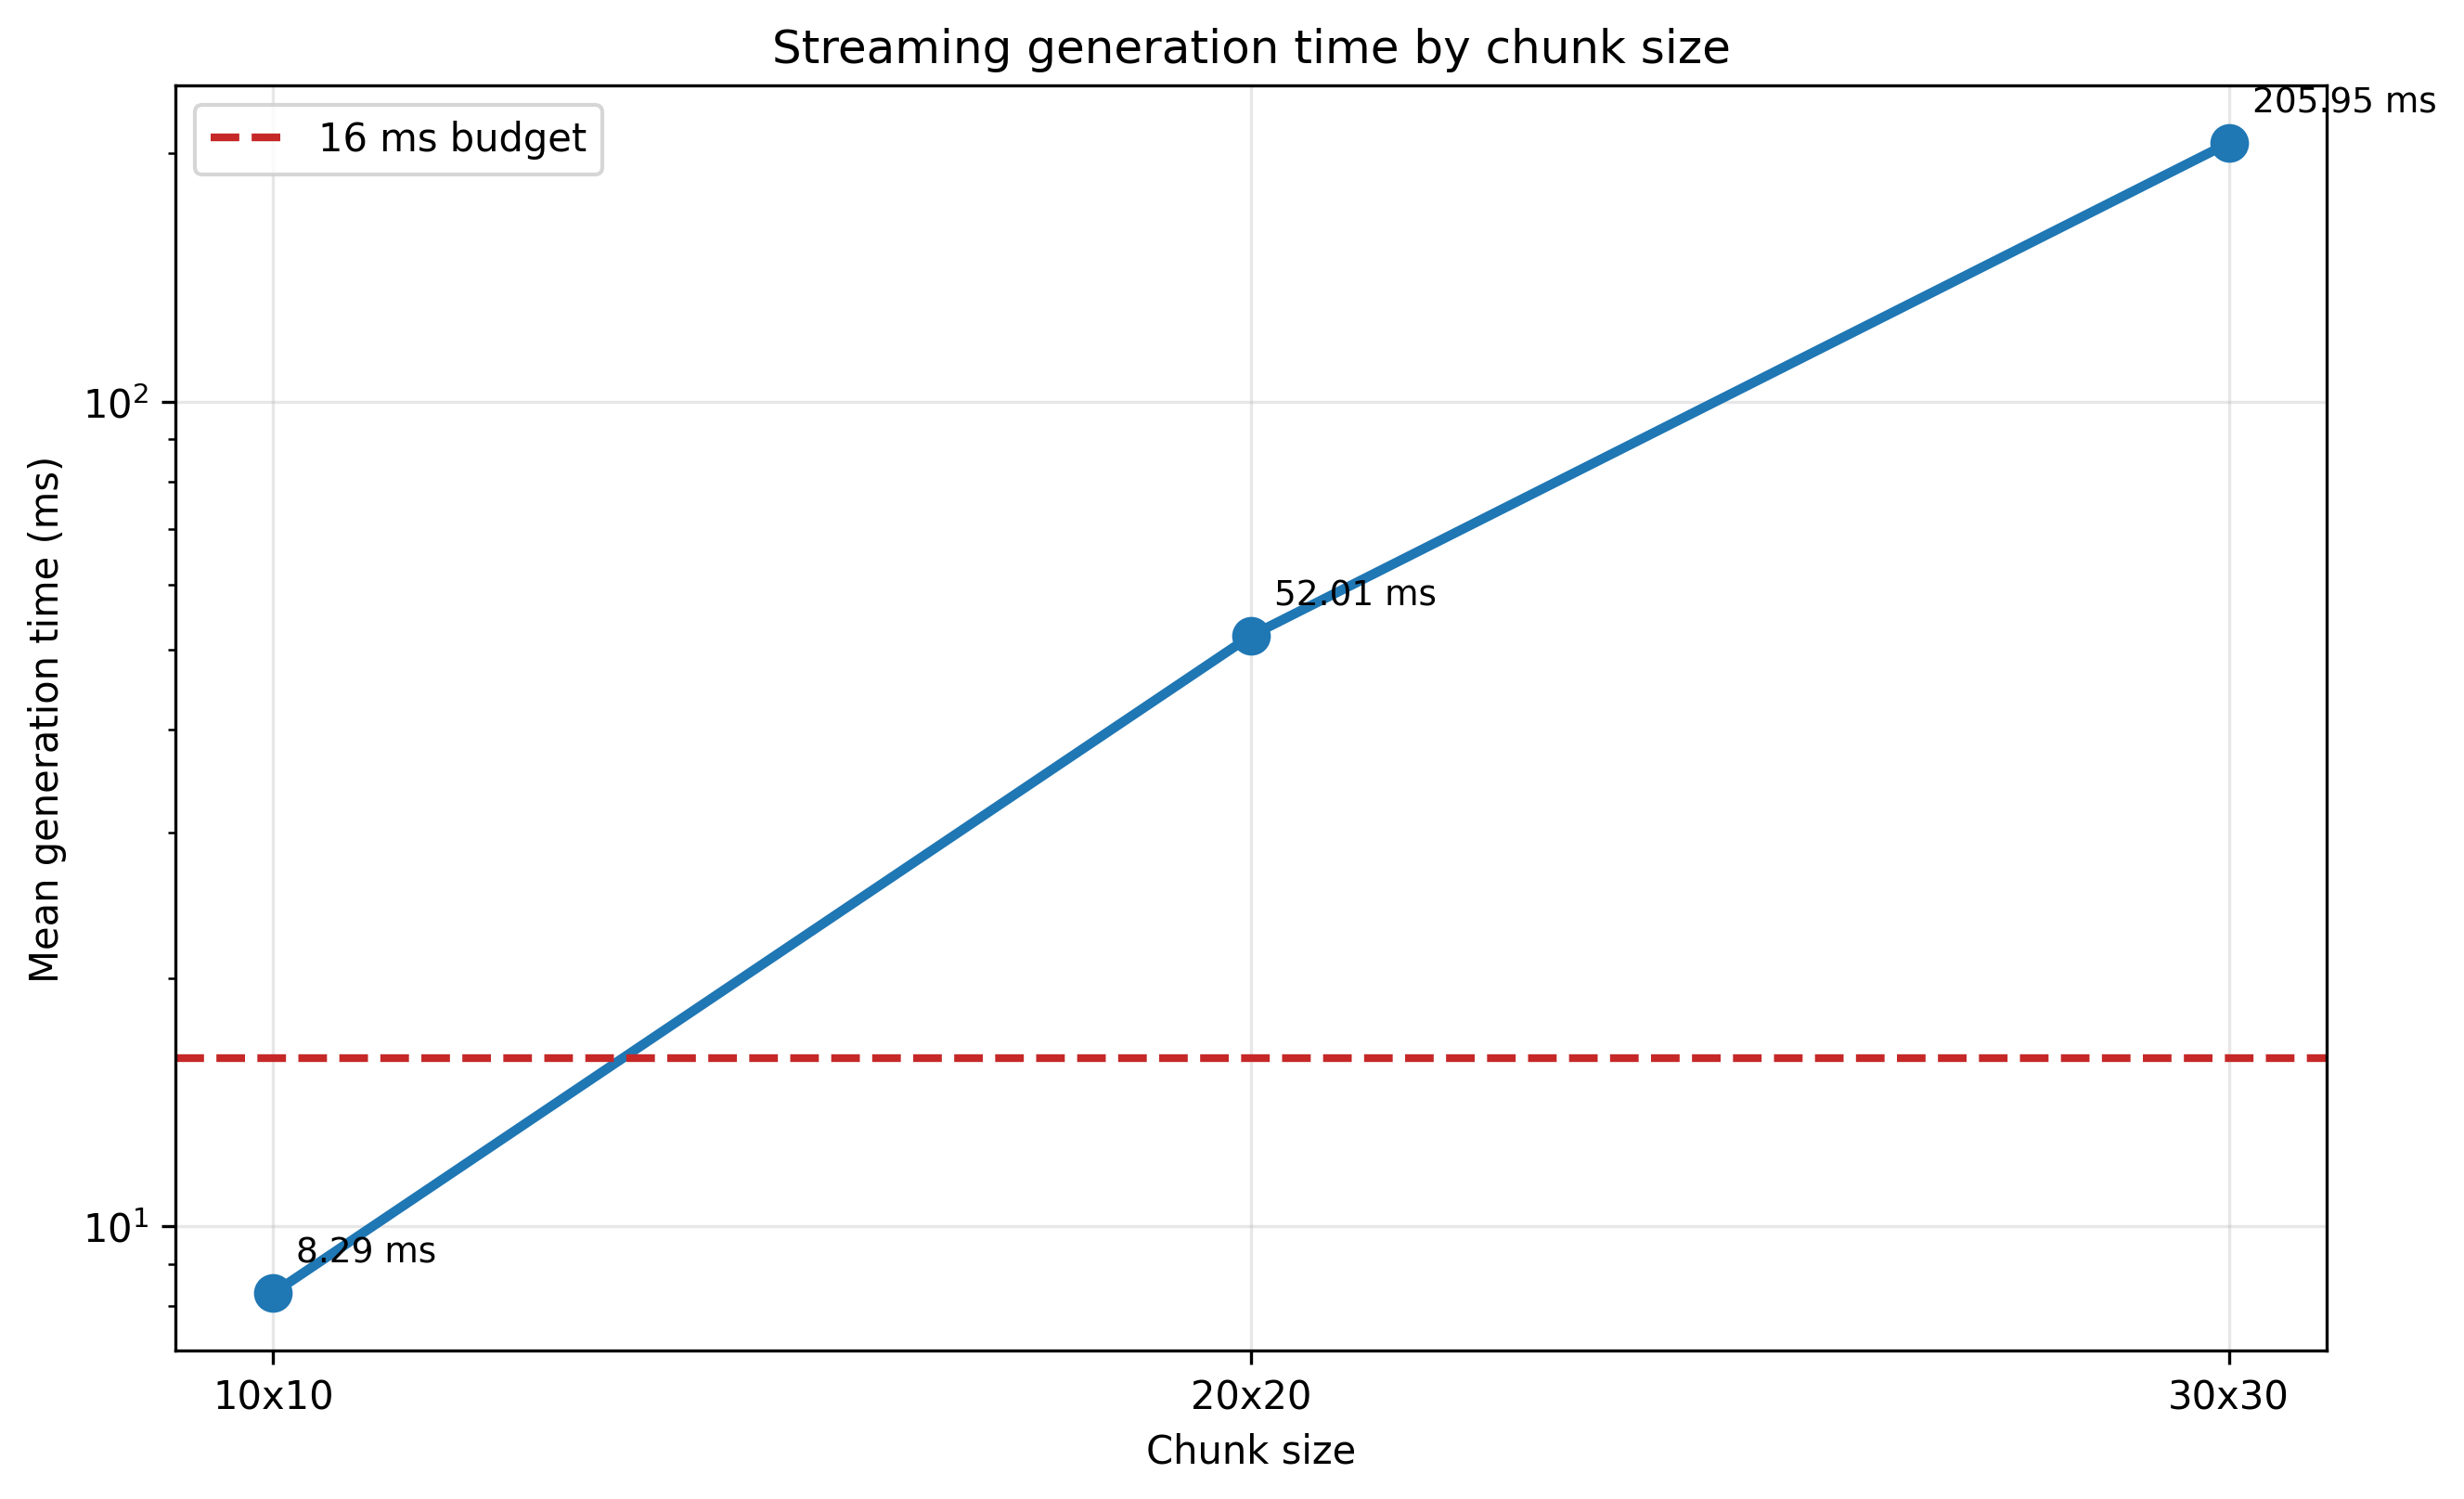
\includegraphics[width=0.85\textwidth]{fig_streaming_timing_growth.png}
\caption{Streaming mean generation time across chunk sizes.}
\end{figure}

\section{Halo Ablation}
The halo ablation results are reported exactly as measured, even though they do not support the original intuition that halo conditioning would dominate the isolated benchmark.

\begin{table}[h]
\centering
\small
\begin{tabular}{rrrrrrrr}
\toprule
Size & $h=0$ succ & $h=0$ mean ms & $h=0$ mean BT & $h=2$ succ & $h=2$ mean ms & $h=2$ mean BT & Context fail \\
\midrule
$10 \times 10$ & 86\% & 2.22 & 0.02 & 84\% & 4.55 & 14.08 & 0 \\
$20 \times 20$ & 84\% & 321.97 & 9218.84 & 68\% & 622.87 & 20807.30 & 0 \\
$30 \times 30$ & 76\% & 686.98 & 11044.62 & 70\% & 895.97 & 13755.24 & 1 \\
\bottomrule
\end{tabular}
\caption{Halo ablation on the fixed target-chunk benchmark. Context failure counts apply equally to both halo settings for the affected trials.}
\end{table}

This ablation indicates that, for the specific capped target-chunk setup used here, halo $h=2$ increased cost and did not improve measured success rate relative to $h=0$. That does \emph{not} invalidate the live streaming system, but it does change the interpretation of the halo mechanism:

\begin{itemize}
\item halo remains part of the final runtime implementation,
\item the current isolated ablation does not demonstrate a net win for halo,
\item future work should test richer boundary contexts and uncapped settings before making stronger claims about halo superiority.
\end{itemize}

\begin{figure}[h]
\centering
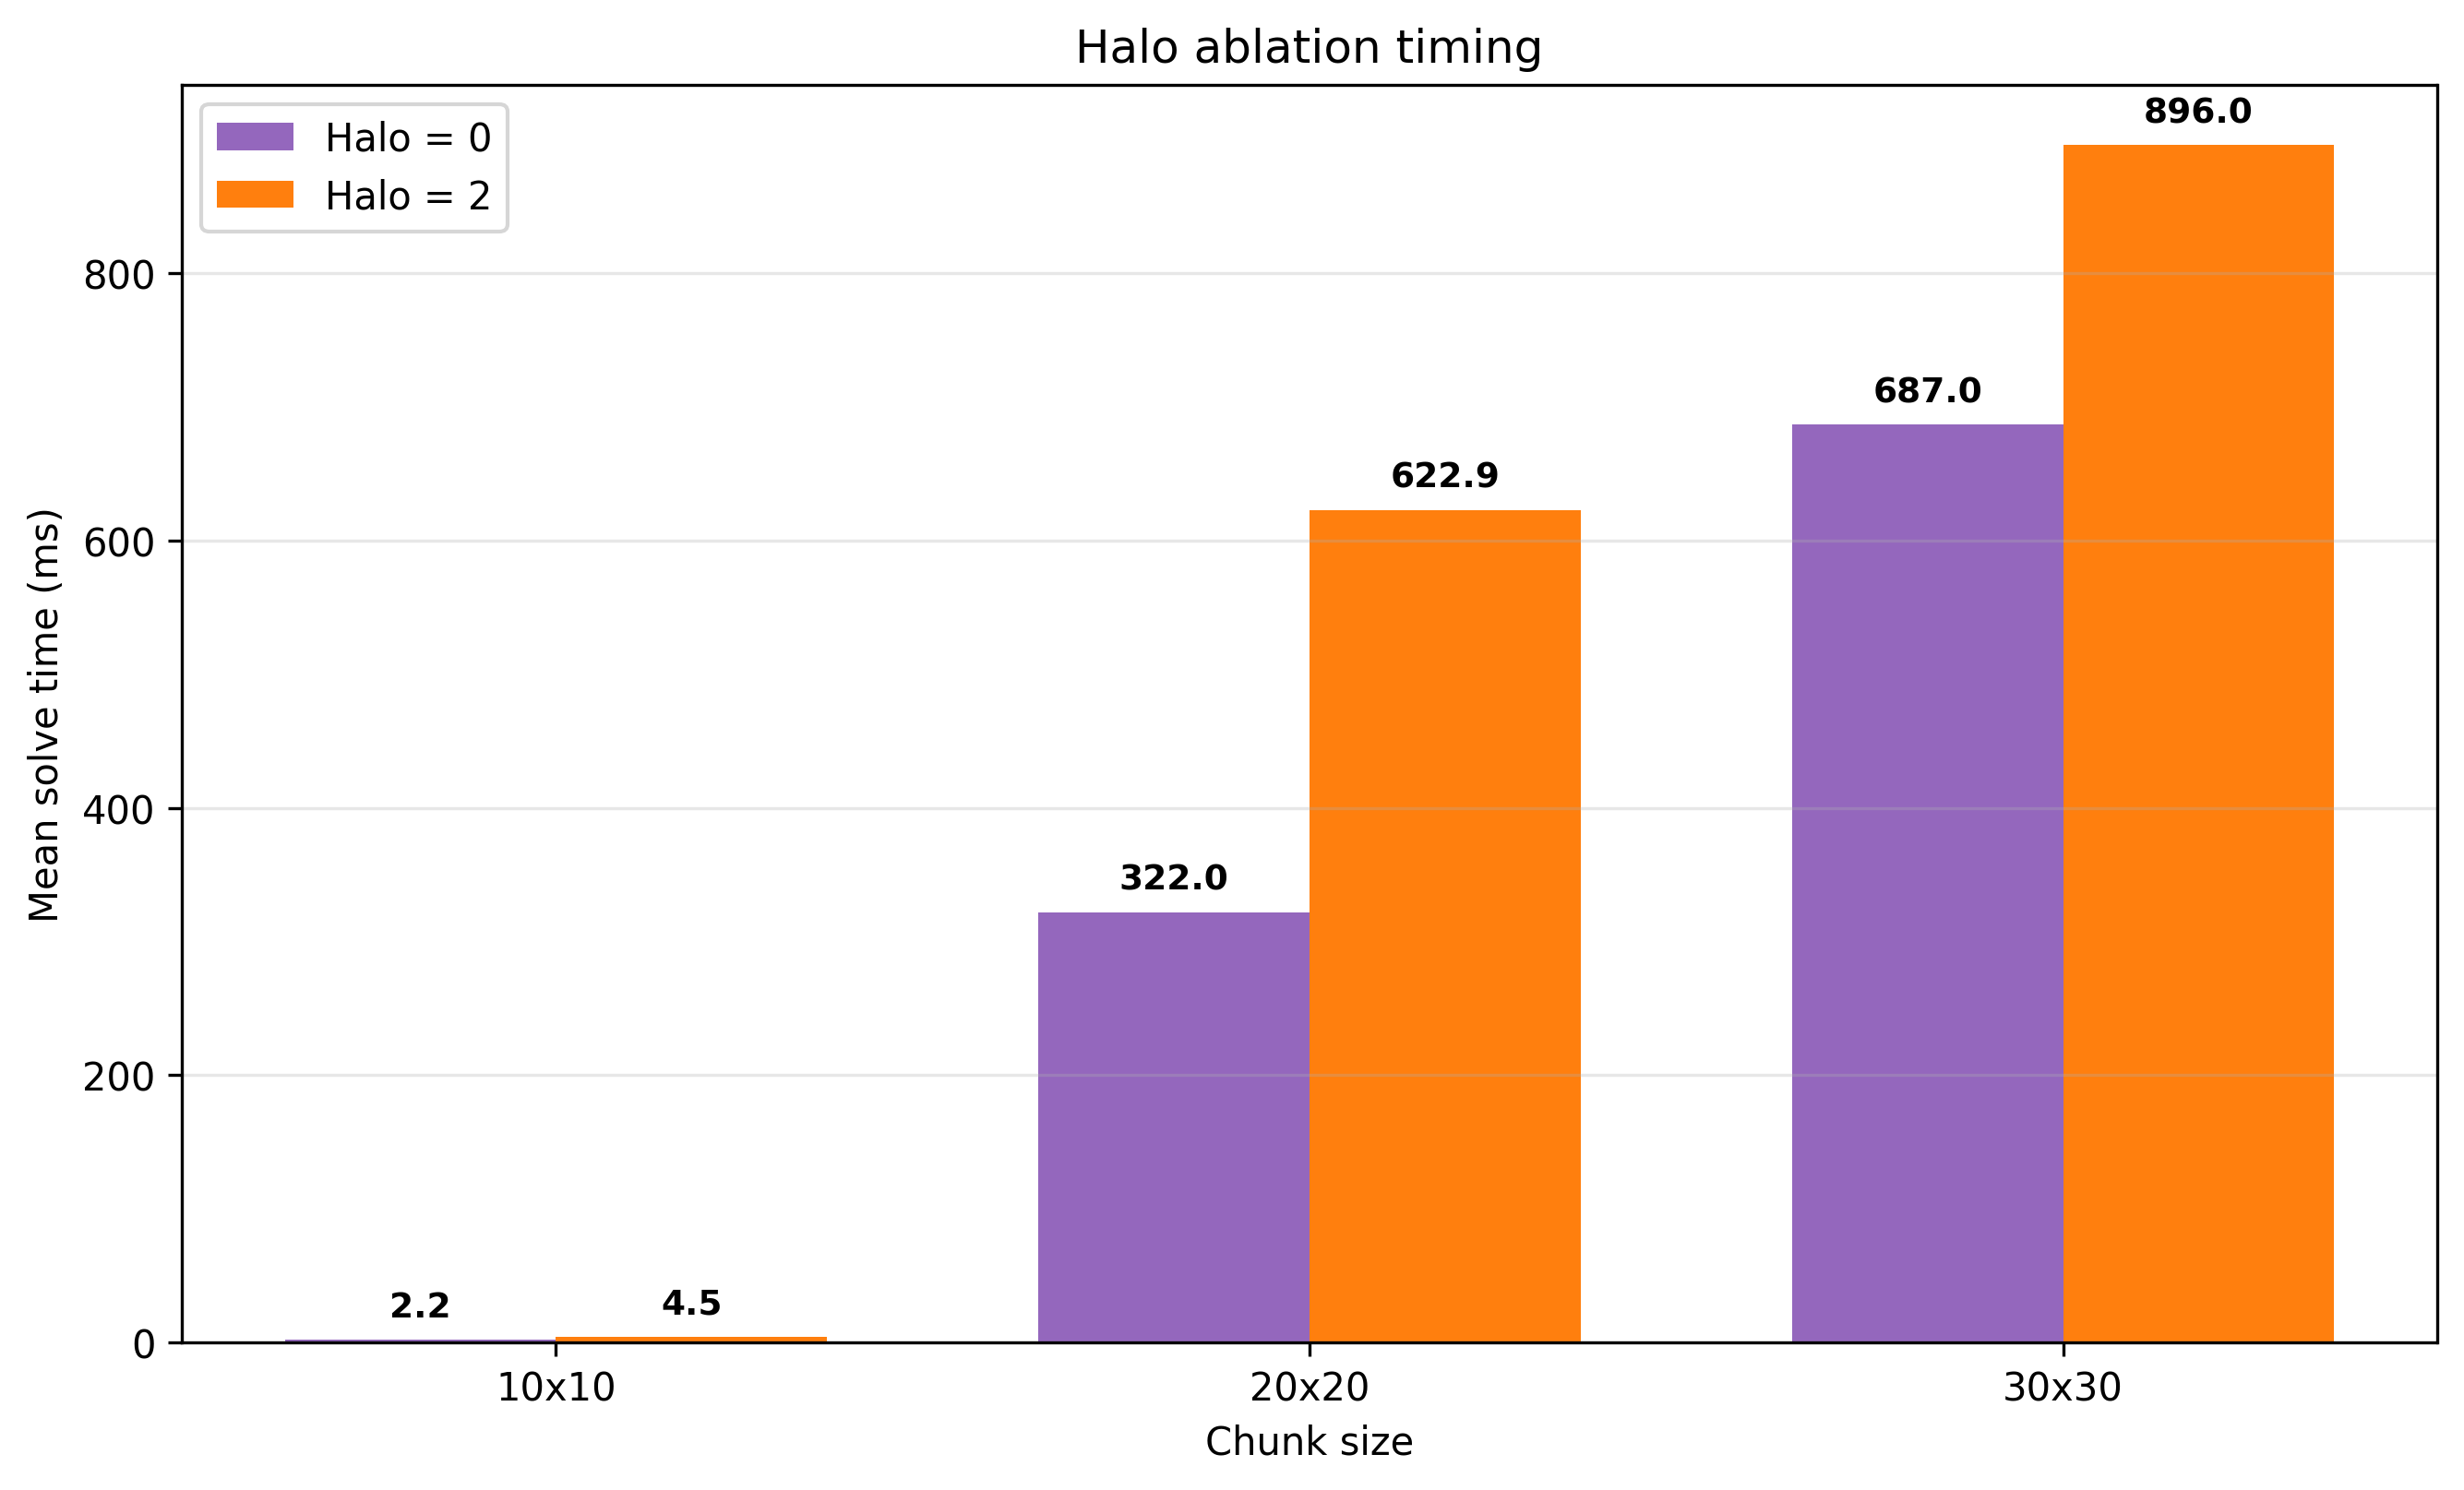
\includegraphics[width=0.85\textwidth]{fig_halo_ablation_timing.png}
\caption{Mean timing cost for the halo ablation benchmark.}
\end{figure}

\chapter{Discussion}
\section{What the Final Package Demonstrates}
The final package demonstrates five strong outcomes.

\begin{enumerate}
\item The cleaned project layout is now presentation-ready and separates runtime code, experiments, figures, and archived drafts.
\item The live browser demo is stable and uses a consistent preset.
\item The solver implementation now matches the intended algorithmic description: explicit change-record undo backtracking.
\item The controlled experiments provide a clear and reproducible restart-vs-backtracking comparison.
\item The streaming experiments validate the system-level claims that matter most for an interactive world: seam correctness, internal correctness, and revisit identity.
\end{enumerate}

\section{What Changed from the Earlier Narrative}
Two earlier assumptions were revised by the final results.

\begin{enumerate}
\item Backtracking is still the preferred live streaming strategy, but on large isolated instances it exhibits a heavy tail and benefits from reporting a timeout rate explicitly.
\item The halo ablation did not show the expected advantage on the chosen benchmark. The final report therefore presents halo as an implemented design component whose isolated value remains an open empirical question.
\end{enumerate}

This is an important part of the project's maturity: the final report is aligned to measured outcomes, not to the proposal's original expectations.

\section{Limitations}
\begin{itemize}
\item The controlled comparison uses a 5 s cap per isolated solve, so the $30 \times 30$ backtracking result should be interpreted as a capped benchmark rather than an unconstrained asymptotic statement.
\item The halo ablation benchmark is intentionally narrow. It compares a fixed target-chunk setting under bounded context generation, not the full live scheduler.
\item The report focuses on one tileset and one deterministic demo seed. Broader tileset diversity would strengthen generality claims.
\end{itemize}

\chapter{Conclusion}
The project is now complete as a masters-level course artifact. It includes a clean repository structure, a working demo, a revised solver implementation, a reproducible experiment bundle, generated figures, and a final report aligned to the actual code.

The final technical conclusion is:
\begin{quote}
Pure backtracking is the right core strategy for the live streaming system, because it preserves a single-search execution model and outperforms restart mode on the controlled benchmark. The streaming system itself is correct in practice on the tested scenarios, with zero seam violations, zero internal violations, and perfect revisit consistency.
\end{quote}

The final research conclusion is slightly more nuanced:
\begin{quote}
Not every implementation hypothesis from the proposal survived empirical testing unchanged. In particular, the halo ablation did not deliver the isolated advantage originally expected. Reporting that honestly strengthens rather than weakens the project, because the final package now reflects measured algorithm behavior instead of proposal-era assumptions.
\end{quote}

This alignment between implementation, experiment, and write-up is what makes the final submission presentable.

\appendix
\chapter{Key Final Numbers}
\begin{itemize}
\item Controlled comparison generated at: 2026-04-09T15:17:38.619Z
\item Backtracking mean time: 3.84 ms (10), 32.28 ms (20), 318.72 ms (30)
\item Restart mean time: 8.53 ms (10), 114.29 ms (20), 867.14 ms (30)
\item Streaming mean time: 8.29 ms (10), 52.01 ms (20), 205.95 ms (30)
\item Streaming correctness: zero seam violations, zero internal violations, revisit passed in all 3 scenarios
\item Boundary-seeding reproduction: direct assignment conflict on tile ids 0 and 1; propagator restriction leaves allowed set \{9\}
\end{itemize}

\end{document}
